
\chapter{Implementation}\label{c:implementation}
Implementation of the conceptualized platform consists of three main parts: The platform hosting the sensors and auxiliary circuitry, a software algorithm for controlling the readout of the sensors and subsequent controlling of the TEC and last but not least software for determining the actual dew point and calculation of other metrics of interest.

\section{Sensor platform}
The sensor platform consists of two printed circuit designs, one base board hosting optical circuitry, power supplies for heating and cooling and connections to the microcontroller, and one mirror board, containing the mirror/capacitor area as well as sensors for temperature readout and circuitry for detecting changes in capacitance.

\subsection{Base board}
The base board is a rigid PCB with dimensions of \qtyproduct{100 x 100}{\mm}. The bottom section includes a voltage regulator for the proximity sensors and an \gls{I2C} bus switch that allows individual sensor operation, despite the sensors sharing the same \gls{I2C} slave address. The right side contains the connections to the external microcontroller platform and to the mirror board. At the top, there are two buck converters that are controlled by \gls{PWM}. In the middle, occupying a \qtyproduct{40 x 40}{\mm} space, lies a cluster of proximity sensors. The layout of these sections enables the creation of an enclosed space with the help of a 3D-printed structure. This enclosure provides mechanical support for the flexible mirror board, shields against external light interference, and offers some control over airflow.

\subsubsection{Proximity sensor array}
The used sensors are Vishay VCNL36825T and Vishay VCNL4040. The main difference between the sensors is the used lighting source, with the Vishay VCNL36825 hosting a \gls{VCSEL} with a pulsed driving current of \qty{20}{\mA} at a peak wavelength of \qty{940}{\nm} and the VCN4040 hosting a infrared \gls{LED} with a driving current of \qty{200}{\mA} at the same peak wavelength of \qty{940}{\nm}. While the laser has a very narrow emitter beam at an angle of about \qty{\pm 4}{\degree}, the \gls{LED} is illuminating a far broader range with an emitting angle of \qty{\pm 15}{\degree}. 

Each sensor type is arranged such, that two sensors are placed in a row, one illuminating the edge of the dew point mirror and one illuminating the center. The VCNL36825T is positioned directly below a temperature sensor on a base board and intended to be used at a distance of at least \qty{50}{\mm} to the mirror surface, while the VCNL4040 sensor is placed with a small shift of \qty{10}{\mm} to the side. Due to the wide angle it is intended to be used at a closer distance.

\subsubsection{Buck Converter}
To effectively utilize the \gls{TEC} and heating traces, power supplies with adequate capacity are essential due to the efficiency of a \gls{TEC} being below \qty{20}{\percent} as outlined in \cref{s:peltier}. This implies that to achieve a cooling effect of \qty{10}{\watt}, a minimum of \qty{50}{\watt} electrical power has to be supplied. Furthermore, the simple relation of $P = R \times I^2$ shows, that for an efficient powering of the \gls{TEC}, a \glslink{PWM}{pulse width modulated} operation of the device with high peak currents should be avoided, in order to minimize thermal losses and thus issues in longevity and heat dissipation.

Hence, a custom buck converter has been designed, which allows a \gls{PWM} controlled operation while giving a stable output voltage. For that a structure consisting of a half-bridge gate driver, two N-channel MOSFETs and a high current inductor alongside a capacitor have been used. The circuit was simulated beforehand in order to make sure, it is able to provide sufficient and stable power at low voltages. The buck converter was placed two times, for the cooler as well as for the heater.

\begin{figure}[!h]
    \centering
    \resizebox{1\textwidth}{!}{%
    \begin{circuitikz}
    \tikzstyle{every node}=[font=\normalsize]
    \draw (0.5,2.5) to[american voltage source] node[pos=0.25,left]{ \normalsize $V_{in}$} (0.5,-1.5);
    \draw [align=right] (6.25,0.5) to[Tnmos] node[pos=-3.5, right]{$N_1$} (6.25,2.5); 
    \draw (5.4,1.5) to[short] (5.25,1.5);
    \draw (6.25,-1.5) to[Tnmos] node[pos=-3.5, right]{$N_2$} (6.25,0.5); 
    \draw (6.25,-1.5) to[short, -*] (6.25,-1.5);
    \draw (5.4,-0.5) to[short] (5.25,-0.5);
    \draw (9.75,0.5) to[short, -*] (9.75,0.5);
    \draw (9.75,-1.5) to[short, -*] (9.75,-1.5);
    \draw (9.75,0.5) to[C,l={ \normalsize $C$}] (9.75,-1.5);
    \draw (6.25,0.5) to[L,l={ \normalsize $L$} ] (9.75,0.5);
    \draw (4.5,2.5) to[short] (6.25,2.5);
    \draw (3.75,-1.5) to[short] (6.25,-1.5);
    \draw (7,0.5) to[short] (6.25,0.5);
    \draw (6.25,-1.5) to[short] (9.75,-1.5);
    \draw (6.25,0.5) to[short, -*] (6.25,0.5);
    \draw (9.75,0.5) to[short, -o] (11,0.5);
    \draw (9.75,-1.5) to[short, -o] (11,-1.5);
    \draw (3.75,-1.5) to[short] (0.5,-1.5);
    \draw (4.5,2.5) to[short] (0.5,2.5);
    \draw  [align=center] (3.25,1.75) rectangle  node {\normalsize Gate\\Driver} (4.75,-0.75);
    \draw (5.25,-0.5) to[short] (4.75,-0.5);
    \draw (5.25,1.5) to[short] (4.75,1.5);
    \draw  (1.75,1.75) rectangle  node {\normalsize MCU} (2.75,-0.75);
    \draw [->, >=Stealth] (11,0.25) -- (11,-1.25)node[pos=0.5,right, fill=white]{$V_{out}$};
    \draw [short] (2.75,0.5) -- (3.25,0.5);
    \end{circuitikz}
    }%
    \caption{Buck Converter for \gls{TEC} and wire heater.}
    \label{c:buck}
\end{figure}

\subsection{Mirror board}
The mirror board is designed as a \gls{FPC} mainly for its low thermal resistance. 

\subsubsection{Mirror and Capacitor}
The copper surface is \gls{ENIG} coated and takes up an area of \qtyproduct{40 x 40}{\mm^2} in the center of the board, matching the size of commonly available TECs.
The area is subdivided for the mirror surface (\qty{23}{\mm}) and the \gls{IDE} capacitor (\qty{17}{\mm}). While the mirror area is a solid plane, the capacitor is designed with a finger width and spacing of \qty{0.1}{mm}, exploiting the minimum manufacturable copper track width and spacing. The length of the fingers is about the edge length with \qty{40}{\mm}. In total, the board hosts 67 fingers. 
% The simulated capacitance of the structure is around TODO F. 


\begin{figure}
    \centering
    % \hspace*{\fill}
    \begin{subfigure}{0.5\textwidth}
        \centering
        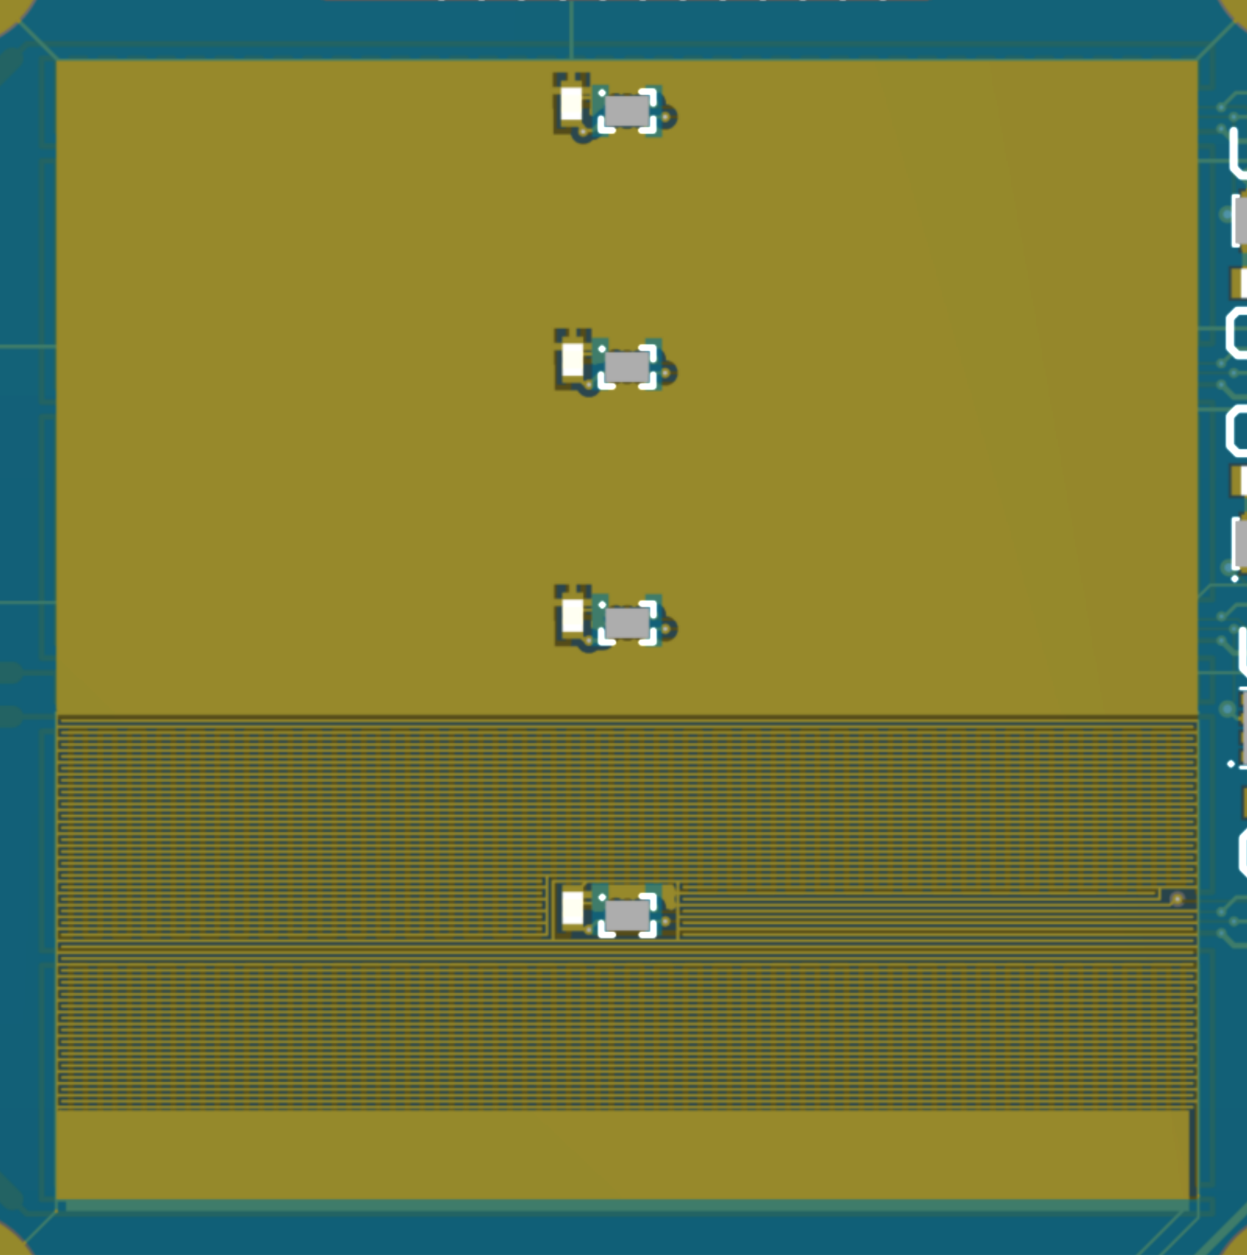
\includegraphics[width=.80\linewidth]{images/flex_mirror.pdf}
        \caption{Mirror and \Gls{IDE} surface} \label{i:mirror}
    \end{subfigure}%
    % \hspace*{\fill}   % maximize separation between the subfigures
    \begin{subfigure}{0.5\textwidth}
        \centering
        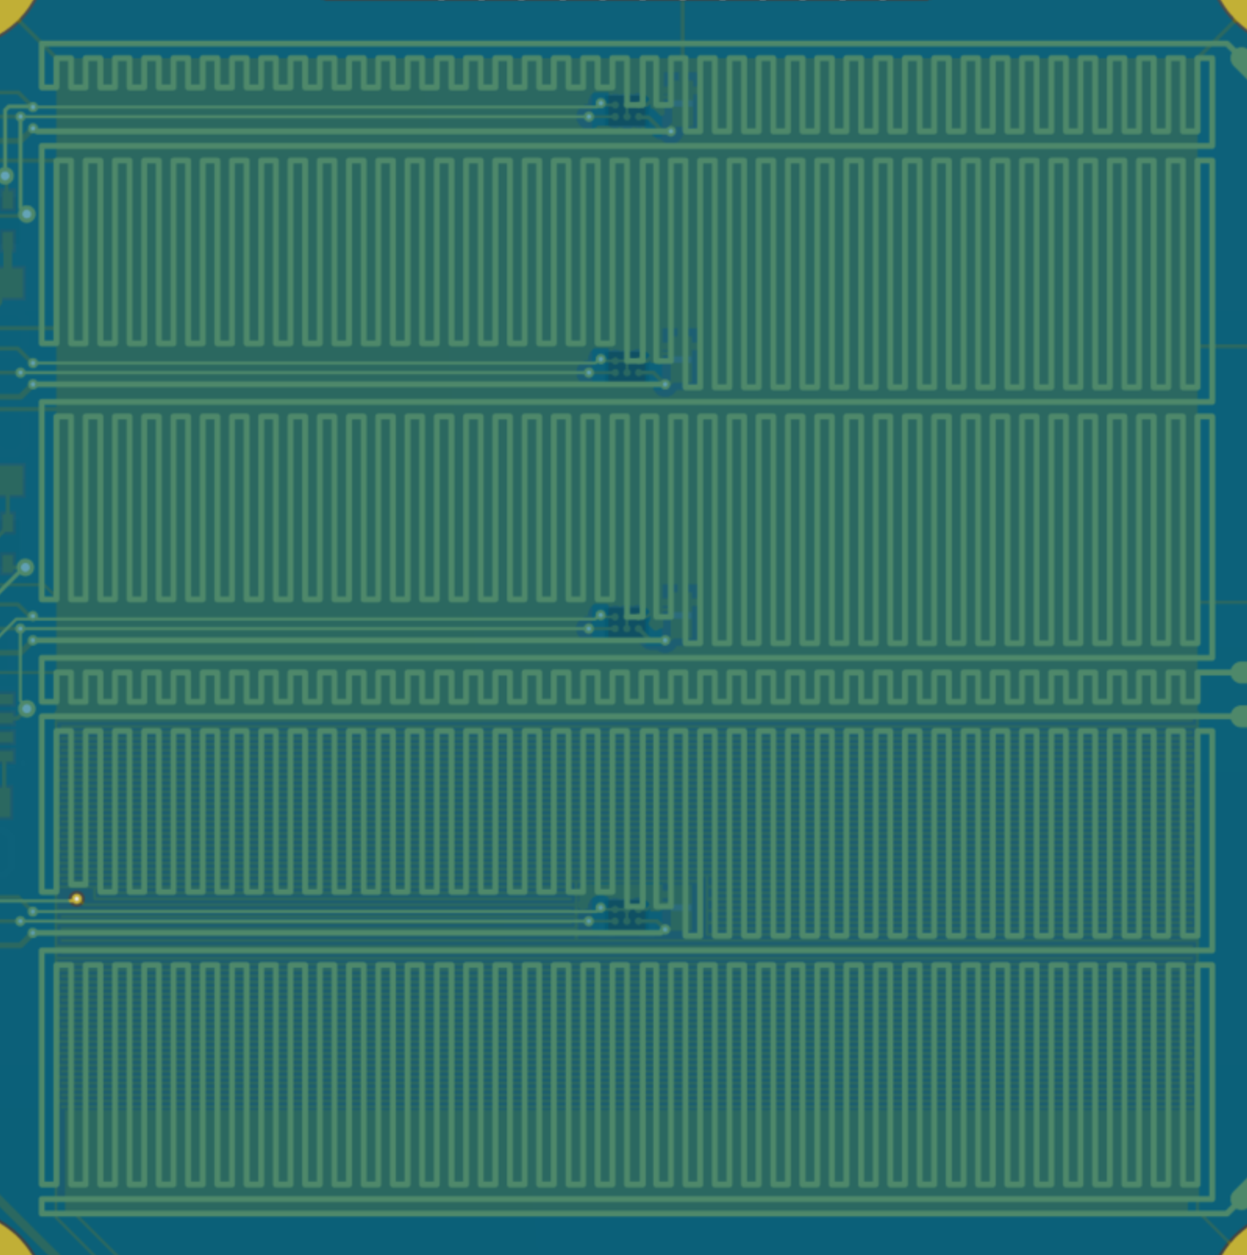
\includegraphics[width=.80\linewidth]{images/flex_heater.pdf}
        \caption{Heater traces} \label{i:heater}
    \end{subfigure}%
  
  \caption{\Gls{FPC} top and bottom layers.} \label{i:mirror_heater}
\end{figure}

\subsubsection{Temperature sensors}
Following the findings of a first concept hosting multiple temperature sensors on the edges of the mirror surface for a comparison in terms of accuracy, responsiveness and mechanical fixture, the final choice of temperature sensors was determined to be Osram AS6221. These temperature sensors are among the smallest commercially available integrated temperature sensors with a footprint of \qtyproduct{1.5 x 1}{\mm}. These small dimensions allow them to be placed directly on top of the mirror surface, giving the benefits of a good thermal coupling and the possibility to compare the temperatures at different locations of the surface. The accuracy of the sensors is specified to be \qty{\pm 0.09}{\celsius} at a range of \qtyrange{20}{42}{\celsius}, being also most accurate among the compared sensors. In total four sensors were placed on the surface, three mainly intended for the optical measurements, two sitting directly above and one above and in between the proximity sensor array. The fourth temperature sensor is placed in the center of the planar capacitor.

\subsubsection{Capacitor readout}
% https://www.electronicdesign.com/technologies/analog/article/21796004/use-analog-techniques-to-measure-capacitance-in-capacitive-sensors
For high accuracy relative capacitance readout, there are various sensing methods available, as briefly described in \cref{s:capacitive_sensors}. The approach implemented in this work is a capacitance-to-frequency converter in form of a so-called relaxation oscillator.

A relaxation oscillator is a type of electronic oscillator circuit that produces a non-sinusoidal output signal, such as a triangle wave or a square wave. The circuit consists of a feedback loop that includes a Schmitt trigger, a resistor, and a capacitor as shown in \cref{c:schmitt}. The Schmitt trigger is a comparator circuit with hysteresis, which means it has two different threshold voltages for switching between its two output states. This hysteresis is commonly used to filter out noise and provide a clean output signal, but in the context of capacitance measurement it can be used to continuously charge and discharge a capacitor, which generates a digital clock signal with a period proportional to the capacitive value being measured.

\Cref{e:cap_charge,e:cap_discharge} describe the charging characteristic of a capacitor by a constant voltage supply $V_{DD}$:
\begin{subequations}
    \begin{align}
        V(t) &= V_{DD} - (V_{DD} - V_{start})\cdot e^{(-\frac{t}{RC})} \label{e:cap_charge}\\
        V(t) &= V_{start} \cdot e^{(-\frac{t}{RC})} \label{e:cap_discharge}.
    \end{align}
\end{subequations}

By inserting $V_{th,p}$ and $V_{th,n}$ as starting and end point conditions for \cref{e:cap_charge} and vice versa for \cref{e:cap_discharge}, the resulting time period for charging and discharging within the threshold voltages can be expressed as:

\begin{equation}
    \label{e:cap_period}
    T = t_{charge} + t_{discharge} = RC \cdot \ln\left[ \frac{(V_{DD}-V_{th,n})V_{th,p}}{(V_{DD}-V_{th,p})V_{th,n}}\right]
\end{equation}

The square wave signal is connected to the microcontroller featuring a capture and compare register, which counts the clock cycles of its internal \qty{172}{\mega\Hz} clock for a signal at an input pin from one rising edge at to the next.

\begin{figure}[]
    \centering
    \resizebox{0.75\textwidth}{!}{%
    \begin{circuitikz}
    \tikzstyle{every node}=[font=\normalsize]
    \draw (5.5,10.75) node[ieeestd invschmitt port, anchor=in](port){} (port.out) to[short] (7.75,10.75);
    \draw (port.in) to[short] (4.75,10.75);
    \draw (4.75,10.75) to[C,l={ \normalsize $C_{IDE}$}] (4.75,9);
    \draw (4.75,12.5) to[R,l={ \normalsize $R$}] (4.75,10.75);
    \draw [](4.75,12.5) to[short] (7.75,12.5);
    \draw [](7.75,12.5) to[short] (7.75,10.75);
    \draw (7.75,10.75) to[R,l={ \normalsize $R_{LP}$}] (10.25,10.75);
    \draw (10.25,10.75) to[C,l={ \normalsize $C_{LP}$}] (10.25,9);
    \draw (4.75,9) to (4.75,8.75) node[ground]{};
    \draw [](10.25,10.75) to[short, -o] (12,10.75);
    \draw [](10.25,9) to[short, -o] (12,9);
    \draw[] (10.25,9) to[short] (4.75,9);
    \draw (7.75,10.75) to[short, -*] (7.75,10.75);
    \draw (10.25,10.75) to[short, -*] (10.25,10.75);
    \draw (10.25,9) to[short, -*] (10.25,9);
    \draw (4.75,10.75) to[short, -*] (4.75,10.75);
    \draw (4.75,9) to[short, -*] (4.75,9);
    \draw [->, >=Stealth] (12,10.5) -- (12,9.25);
    \draw [short] (12.25,9.5) -- (12.5,9.5);
    \draw [short] (12.5,9.5) -- (12.5,10.25);
    \draw [short] (12.5,10.25) -- (12.75,10.25);
    \draw [short] (12.75,10.25) -- (12.75,9.5);
    \draw [short] (12.75,9.5) -- (13,9.5);
    \draw [short] (13,9.5) -- (13,10.25);
    \draw [short] (13,10.25) -- (13.25,10.25);
    \draw [short] (3.75,10.5) -- (4,10.75);
    \draw [short] (4,10.75) -- (4.25,10.5);
    \draw [short] (4.25,10.5) -- (4.5,10.75);
    \end{circuitikz}
    }%
    \caption{Relaxation oscillator using Schmitt trigger for capacitance sensing.}
    \label{c:schmitt}
    \end{figure}

\subsubsection{Heater}
The heating element is placed on the other side of the FPC, directly on top of the mirror and capacitor, sharing roughly the same dimensions. Its use is to give another degree of freedom in temperature control, for example in order to control the speed of evaporation in case of formed dew or to raise the temperature in case of high relative humidity.

The trace heater is designed to provide a uniform heating rather than providing large amounts of heat, hence the trace width and spacing has been chosen to be rather small with \qty{0.2}{\mm} and \qty{0.3}{\mm} respectively. The resulting coil like formation as seen in \cref{i:heater} has a total length of \qty{545}{\mm} with the possibility to manually split the connection in order to heat the area of the mirror and the area of the planar capacitor individually. 

\subsubsection{Physical setup}
\Cref{i:sensor_flex,i:sensor_rigid} show the physical setup of the two components of the system. The base board is mounted on a 3D printed mount for levelling and spacing to the ground, with an additional fixture for the STM32 development board.
Another 3D printed structure on top allows for spacing and adjustment of the mirror/capacitor \gls{FPC}. It is designed to put the \gls{FPC} aligned to the proximity sensors of the base with a vertical spacing of \qty{22}{mm}.


\begin{figure}[hb!]
    \centering
    % \hspace*{\fill}
    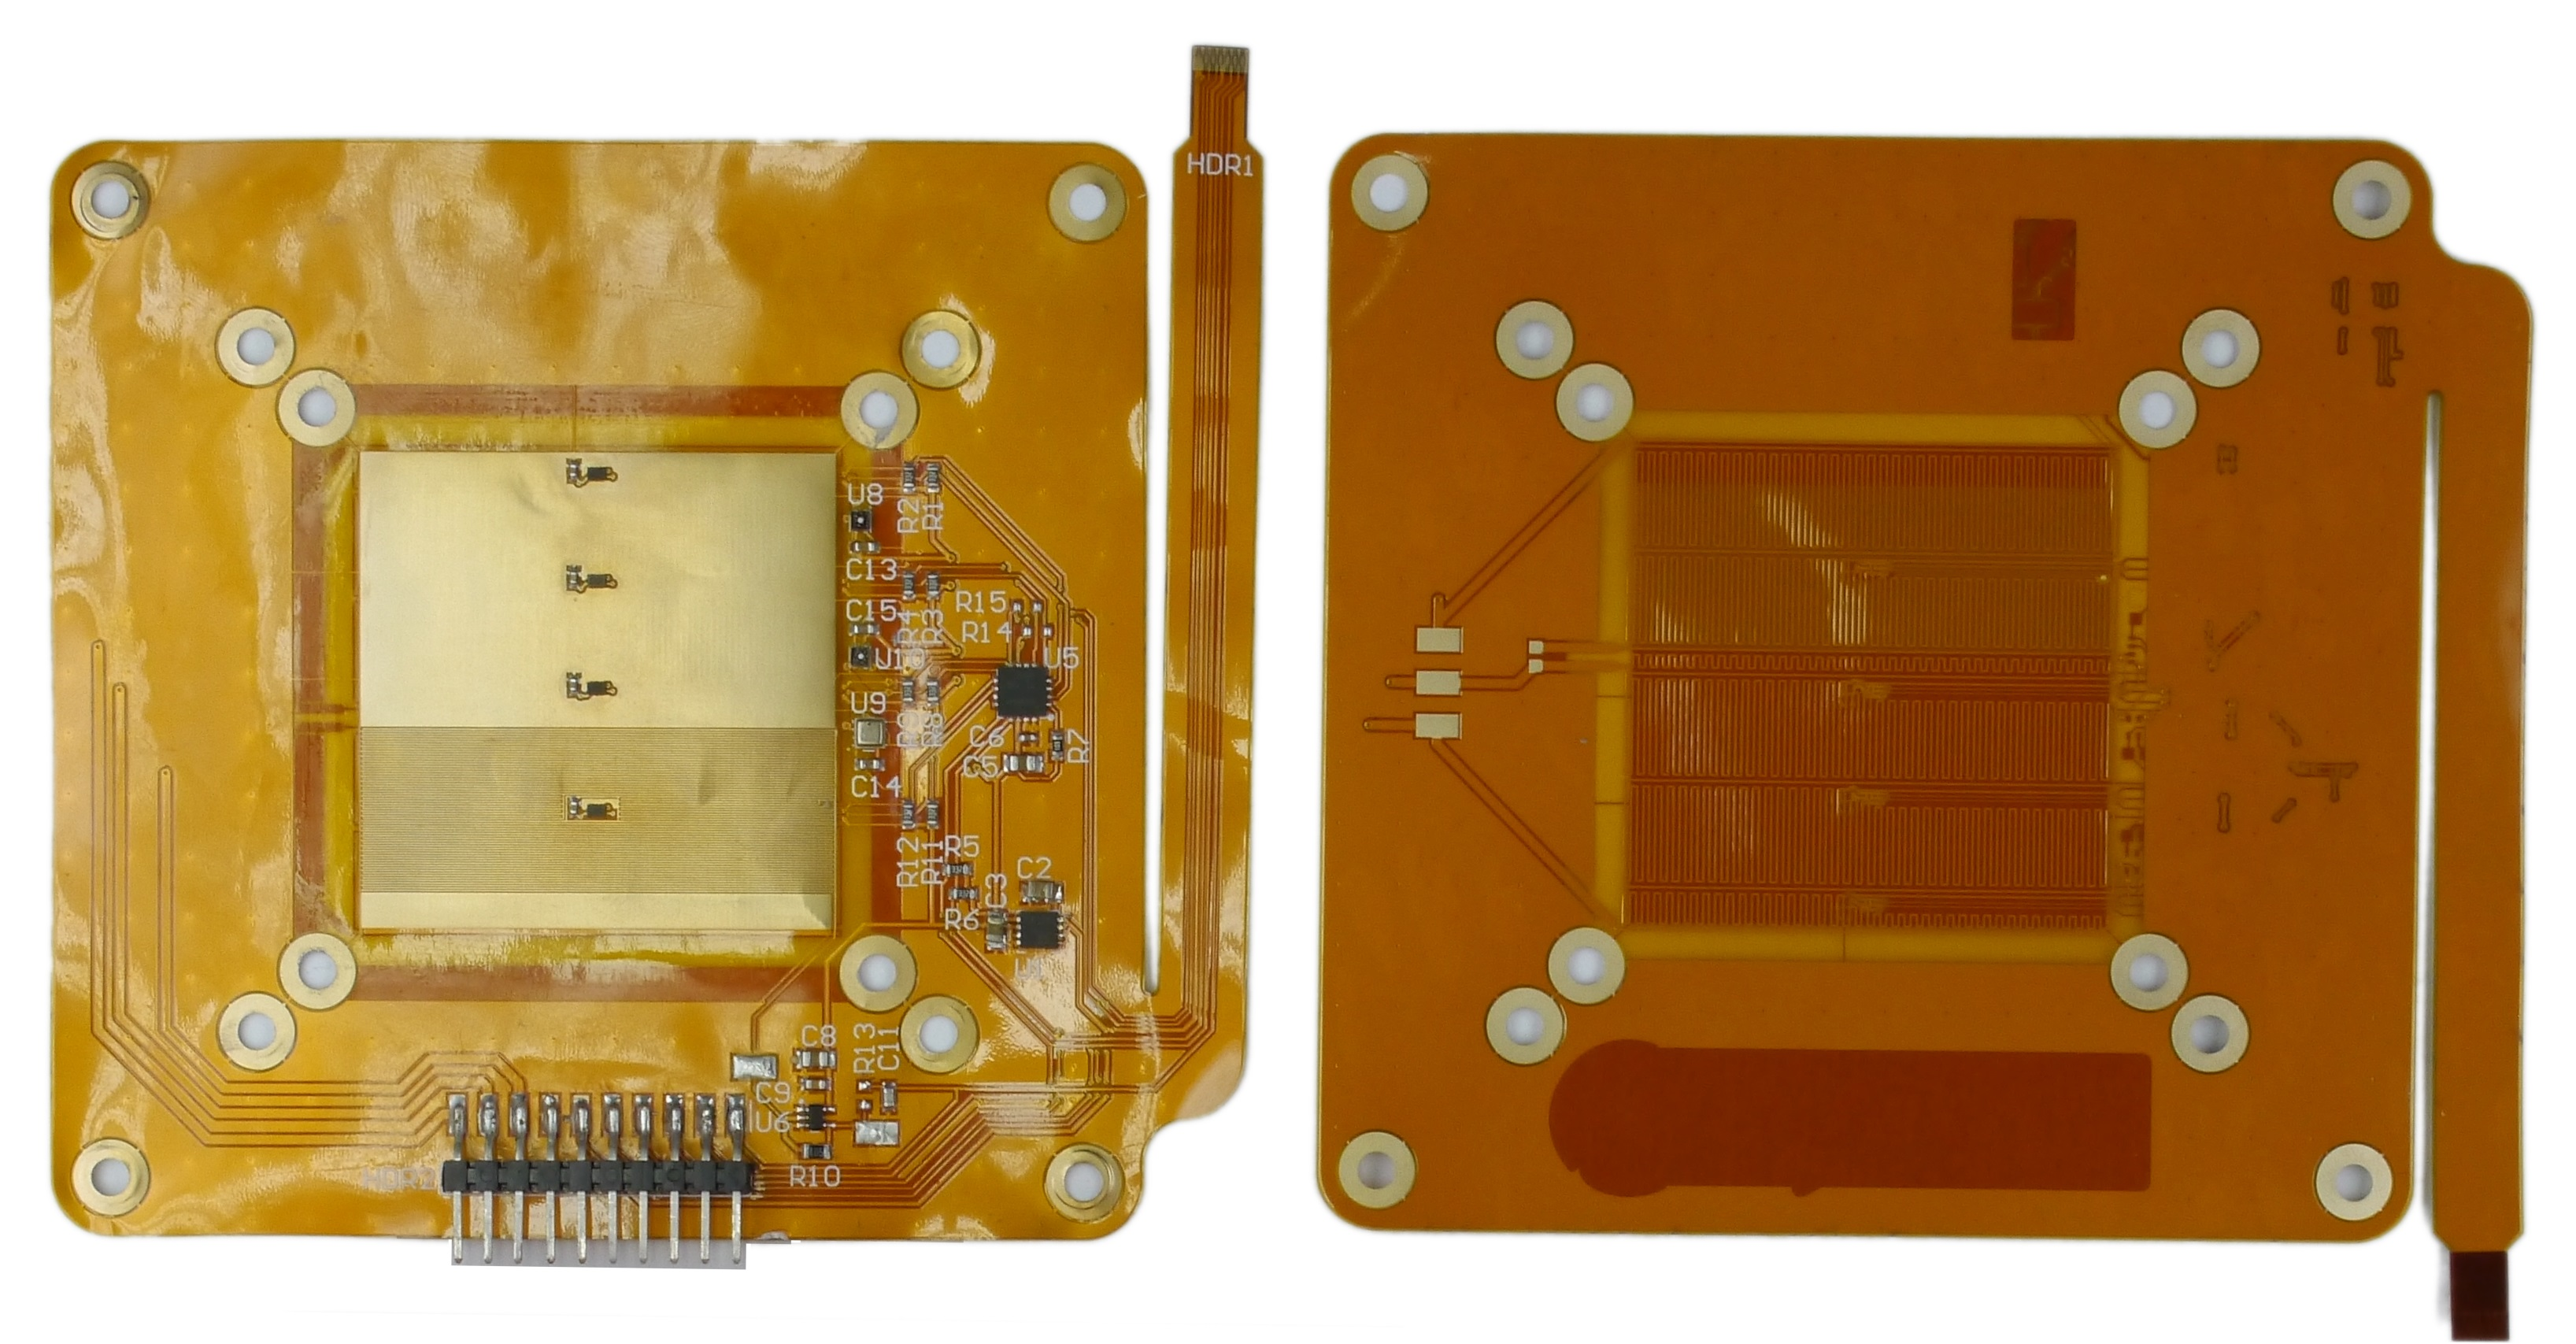
\includegraphics[width=0.9\linewidth]{images/sensor_flex1.jpg}
    \caption{Photograph of the mirror/capacitor \gls{FPC} front and back.}
    \label{i:sensor_flex}
\end{figure}

\begin{figure}[ht!]
    \centering
    % \hspace*{\fill}
    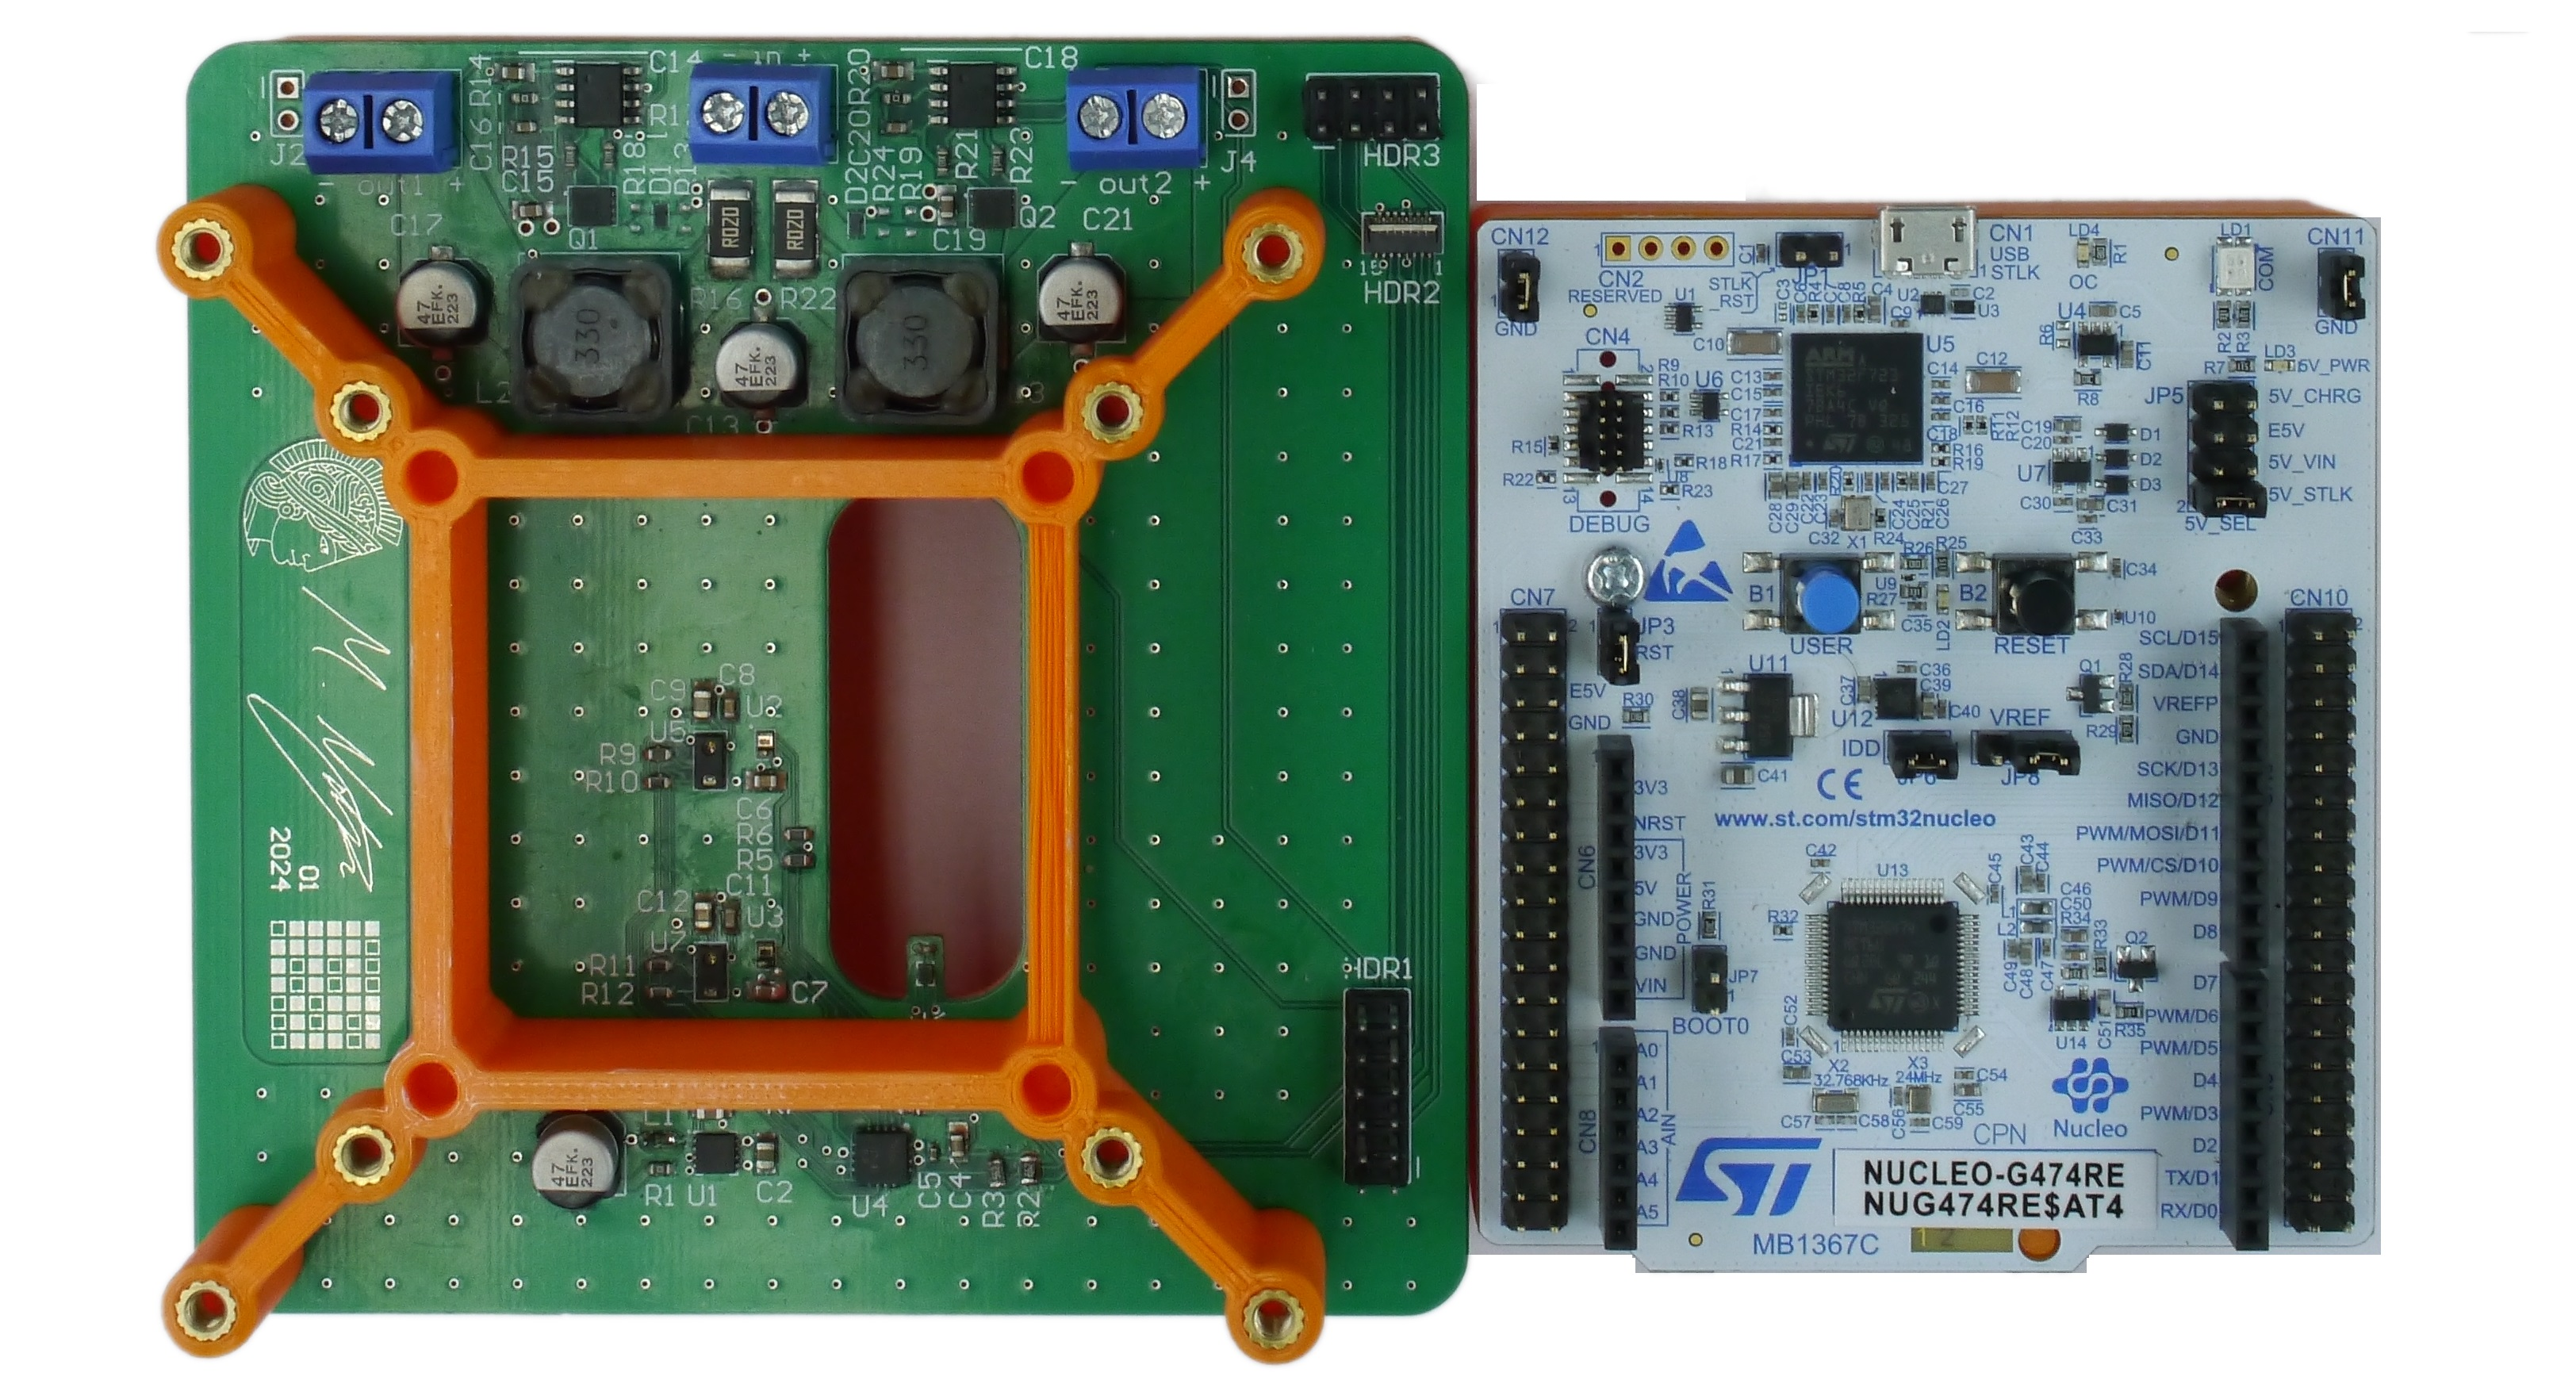
\includegraphics[width=0.9\linewidth]{images/sensor_rigid1.jpg}
    \caption{Photograph of the base \gls{PCB} alongside the STM32 microcontroller \gls{FPC}.}
    \label{i:sensor_rigid}
\end{figure}

\section{Control software}\label{c:control}
As explained in \cref{s:background,s:concept}, the measurement of the measurement principle of the chilled dew point hygrometer requires a cooling of the sensed mirror/capacitor surface.
In order to guarantee correct measurement of the dew point, an algorithm for controlling the sequence of measurement steps is therefore inevitable. As the cooling needs to be performed for a wide variety of temperature ranges and possibly requires a large change in temperature, there is a need for an estimation of the dew point temperature. Without such analysis, the measurement and energy consumption is either excessive in the case of cooling down to the lowest temperatures feasible, or otherwise potentially not sufficient, if the target temperature or cooling duration is not sufficient for reaching the dew point.
The exact analysis of dew point however is performed on an external computer after completion of the measurement cycle with methods described in \cref{c:readout}.

The software for performing the measurement cycle is written stm32duino, a software platform implementing the Arduino API for the STM32 microcontroller platform. Only a minor fraction of the code makes direct use of the officially provided hardware abstraction layer from STMicroelectronics in order to access certain hardware timer functionality. This yields the benefit of fast prototyping and cross-manufacturer compatibility requiring only minor code changes for adaption in different microcontrollers.
\clearpage
\begin{wrapfigure}{r}{0.5\textwidth}
    \centering
    \def\svgwidth{0.365\textwidth}
    \input{drawings/control2.pdf_tex}
    \caption{Control sequence}
    \label{d:control}
    \vspace{-55pt}
\end{wrapfigure}

The initiation of a measurement is performed using a host computer connected over a serial connection to the STM32 microcontroller. Different commands are provided for enabling and disabling sensors, for performing sensor readouts and most importantly for initiating the measurement cycle as seen in \cref{d:control}.

The cycle starts by setting initial conditions, such as the sensing period, the amount of repetitions and the desired temperature slopes. This leads to the entering of the control loop, which is periodically performed according to the set period. The loop first disables both cooling and heating \gls{PWM} outputs. This step is performed in order to avoid the possibility of noise introduction, especially in measurement of the capacitance, due to switching of the half bridge \glspl{MOSFET} and ripple within the \gls{TEC} and heater. 

After that, all measurements on the provided list of enabled sensors are initiated, in a parallel manner for the temperature as well as reference humidity and pressure sensors and in a sequential manner for optical and capacitive sensors. This distinction is required in order to avoid mutual interference. The complete measurement time depends on the amount and type of enabled sensors and can be expressed as 
\begin{align*}
    t_{meas} = \max \{ &\max \{t_{temp}, t_{press}, t_{hum}\}, \\
    &t_{cap} + \sum t_{prox} \}
\end{align*}
The sensors are set to measure with maximum precision wherever possible, leading to measurement times of \qty{36}{\ms} for the temperature sensors, \qty{5}{\ms} and \qty{7}{\ms} for the VCNL36825T and VCNL4040 proximity sensors, and up to \qty{10}{\ms} for the capacitor sensor. The measurement times for reference humidity and pressure sensors are in the range of \qty{10}{\ms}.

After the measurement is finished, the \gls{PWM} is turned back on and the data of the sensors is fetched. Based on the current state, the next state is determined. The state changes, if either a temperature or a capacitance limit has been reached and subsequently the temperature slope, a term of $\Delta T / s$, is updated. In the first iteration of the loop, the lower and upper boundaries for capacitor values are determined by a percentual factor of the initially measured capacitance. This is needed, in order to limit the cooling and heating duration as described above. \Cref{c:results} describes the governing physi-chemical mechanisms used for this. The temperature limits for reheating and recooling are set after the dew point was detected for the first time using the relative capacitance term.

In the following step, the temperature setpoint is determined using the actual setpoint and the offset defined by the slope. Using the temperature error, defined by the difference of measured temperature and the setpoint, the pulse width of the \gls{PWM} signal is updated by a control loop mechanism in form of a \gls{PID} controller. The controller determines a set value using the following terms:
\begin{itemize}
    \item Proportional: Produces and output value that is proportional to the current error value.
    \item Integral: Accumulates past errors over time to eliminate offset and steady-state errors.
    \item Derivative: Uses the rate of change of the error in order to accelerate the response in an abrupt system change and oscillations.
\end{itemize}
The heater was not provided with a seperate PID controller, as it only serves as a supporting system, that limits the amount of condensation on the sensor and thus decreases the time required for evaporation of dew. Its value is determined relative to cooler PID controller and is only applied in a reheating state.

The resulting pulse widths are set accordingly and all relevant data is transmitted to the host computer for dew point analysis and logging purposes. Among this data is every sensor reading, as well as the current state, temperature setpoints and errors and \gls{PID} controller values.

Finally, the state machine either proceeds with the next loop iteration after a delay of the remaining duration of the measurement period, or it finishes operation, if the last state is completed.

%Diagram exemplary response

\section{Data readout}\label{c:readout}

In the field of signal analysis, the selection of data filtering is crucial as high frequency noise can significantly impact the identification of points of interest, particularly in the presence of hard short term flanks. This issue becomes even more critical when numerical derivations need to be performed. While a linear interpolation of the original samples can be visually categorized in terms of trends, digital processing using linear interpolations of numerically derivated samples may be impossible due to abrupt changes in the slopes. To address these challenges, a variety of filters and regression techniques exist, such as finite impulse response (FIR) filters, infinite impulse response (IIR) filters, and polynomial regression methods like smoothing splines or LOESS. Commonly used filters are finite impulse response filters, which are a class of low pass filters that reduce high frequency noise. Notable implementations of FIR filters include simple moving average and weighted moving average. In a simple moving average, all samples of a filter are equally weighted using a boxcar function (also referred to as a rectangle window). In contrast, a weighted moving average assigns different weights to parts of the window, giving them higher importance. However, these filters are rather inflexible and need to be tuned accordingly. Large window sizes lead to overdampening, making it impossible to detect edges, while small values are ineffective at counteracting noise. Additionally, response time is severely slowed down and behavior at the start and end of measurement differs. 

For these reasons, a regression method, specifically smoothing splines, was chosen for this study with the primary intent to obtain reliable results in numerical derivation. For regression, a large variety of functions and approximation methods have been studied. A very versatile approach is the use of piecewise connected polynoms of a specified degree $k$, also called B-splines. For an array of $n$ samples, B-splines are globally continuous up to the $(k-1)$th derivative and defined by coefficients and knots. The coefficients are used in conjunction with localized polynomials, also called basis elements, which the B-spline is made up of:

\begin{equation}
    s(x) = \sum_{i=-k}^{n} c_i  N_{i, k}(x)
\end{equation}

The set of basis elements $\{N_{i,k}\}^n_{i=-k}$ are associated to the knot vector $T = \{t_{-k}, t_{-k+1}, ...,\\t_{n+k+1}\}$, consisting of a knot at each sample and additionally introduced boundary knots, and defined recursively by the Cox-de-Boor formula:

\begin{subequations}
    \begin{align}
        N_{i, 0}(x) &= \begin{cases}
            1,& \text{if } t_i \le x < t_{i+1} \\
            0,& \text{otherwise}
        \end{cases}\\
        N_{i, k}(x) &= \frac{x - t_i}{t_{i+k} - t_i} N_{i, k-1}(x)
        + \frac{t_{i+k+1} - x}{t_{i+k+1} - t_{i+1}} N_{i+1, k-1}(x)
    \end{align}
\end{subequations}

The formula shows, that the basis elements are linear combinations of usual monomials $x^m$  with $m = 0, 1, ..., k$ with the special feature, that they equal to zero outside an interval defined by a knot array consisting of $k + 2$ knots.
    
The amount and placement of knots defines the fitting of the curve, i.e. for the maximum amount of $n + 2k + 1$ knots, the spline completely satisfies the input array, resulting in a polynomial interpolation. In order to find a spline, i.e. its knots and coefficients, that fits the data with a variable amount of smoothing, the algorithm proposes a scheme, where the discontinuities in the $k$th derivative are to be minimized:
\begin{equation}
    \sum_{r=k+2}^{n-k-1} \left[ s^{(k)}(t_r + 0) - s^{(k)}(t_r - 0) \right]^2,
\end{equation}

while an error constraint with a passed smoothing parameter $s$ is fulfilled:
\begin{equation}
    \sum_i \left[ w_i (g(x_i) - y_i)\right]^2 \leqslant s.
\end{equation}

For a smoothing parameter equal to zero, each knot has to be traversed, leading to a high amount of discontinuities in the derivative, whereas for a sufficiently large smoothing parameter, the amount of knots will be minimal, possibly leading to an approximated curve in the form of a straight line.

In order to make use of this powerful tool, the implementation provided by the scientific computation library scipy was chosen for dew point analysis.